\documentclass[../main.tex]{subfiles}


\begin{document}

\chapter{Approach}
\label{chap:approach}

This chapter covers the description, justification, and realization of the protocol that encrypts logs in the toolchain.
In the previous chapter \ref{chap:overview}, possible solution strategies were introduced and evaluated based on the identified system requirements in chapter \ref{chap:requirements}.

Section \ref{sec:justification} summarizes the previous analysis and justifies why hybrid encryption is the most promising approach in the context of this thesis.
This selection fixes the fundamental encryption techniques of the protocol.
To comply with the requirements, however, the designed protocol not only performs encryption but also contains cryptographic signatures.
The description of the implemented encryption and decryption algorithms can be found in \ref{sec:protocol-design}.
Besides the theoretical outline of the implemented protocol, this chapter also details the corresponding libraries and packages that were developed in the scope of this thesis.
Those libraries are implemented in three programming languages (Typescript, Python and Go).
This ensures that different software components can handle logs as specified by the protocol.
Details about this practical realization of the libraries can be found in section \ref{sec:implemented-libraries}.
Moreover, the chosen approach heavily influences the existing toolchain.
The existing source code of the toolchain was therefore refactored and adjusted to handle E2EE logs.
This is described in detail in section \ref{sec:toolchain-modifications}.

\section{Hybrid encryption}
\label{sec:justification}
The protocol introduced in this chapter relies on hybrid encryption.
The purpose of this section is the justification of this encryption technique.
Recall table \ref{tab:overview-summary} in chapter \ref{chap:overview}, where different approaches were evaluated under the given requirements.
The table visualizes the fulfillment of the requirements of each considered approach.
Hybrid encryption satisfies all functional and security requirements.
Only the non-functional performance criterion N4 can not be fully met because the symmetric key needs to be encrypted for all receivers.
The following argumentation illustrates why hybrid encryption is nevertheless the most promising approach.

First of all, hybrid encryption improves mutual encryption because it avoids encrypting application data with asymmetric cryptography.
Instead of encrypting a log multiple times under different public keys, hybrid encryption applies fast symmetric algorithms to encrypt the log.
It then additionally encrypts the symmetric key under the public keys of the receivers.
This adheres to currently proposed best practices in applying cryptography~\cite[340]{Eckert2018}.
The performance difference might not be noticeable in the current protocol because the encrypted logs do not contain a lot of information.
However, the usage of hybrid encryption ensures that the encryption is still performant if the logs are extended in the future.
Notice that there is no difference in terms of security and functionality between the approaches.
Thus, hybrid encryption outperforms mutual encryption.

Another option to implement the intended protocol is based on broadcast encryption techniques that encrypt data for multiple receivers.
As elaborated in section \ref{sec:broadcast-encryption}, different approaches are proposed to implement broadcast encryption.
In general, there is no need to encrypt data $n$ times when it needs to be decrypted by $n$ users in those schemes.
Considering the non-functional criterion N4 (minimal resource utilization), broadcast encryption, therefore, outperforms hybrid encryption.
The main disadvantage of broadcast encryption is the missing standardization.
Specifically, the Web Cryptographic API does not include any of those schemes.
Thus, they can only be used in the browser if the reference implementations are translated into Javascript.
Since Javascript is an interpreted language, however, this comes with considerable performance limitations.
Moreover, the cryptographic library implemented in this thesis needs to be delivered in three programming languages.
Translating a dedicated scheme into multiple languages is complex, error-prone, and not realizable within the time constraint of this thesis.
Please also notice that each approach introduced in section \ref{sec:broadcast-encryption} additionally suffers from security limitations undermining the understanding of E2EE.
Since hybrid encryption relies on standardized and well-researched algorithms, it is preferred over broadcast encryption techniques.

A third option is an implementation based on a key server.
The log is encrypted with a symmetric scheme and access to the decryption key is maintained by a key server.
This approach only relies on well-researched symmetric encryption techniques.
It can therefore be implemented in different programming languages and environments.
A key server, however, introduces key escrow which harms the intended E2EE.
This is a major drawback compared to hybrid encryption.

\section{Protocol design}
\label{sec:protocol-design}

This section details the implemented protocol which is based on hybrid encryption to enable E2EE.
The evaluation in terms of functionality, security, and performance can be found in chapter~\ref{chap:evaluation}.
The designed protocol internally uses the \textit{JSON Object Signing and Encryption} standard (\textit{JOSE})~\cite{Barnes2014}.
Details about it can be found in section~\ref{sec:jose}.
\textit{JOSE} defines encryption and signature standards that can be used to create a protocol satisfying all system requirements.
A high-level overview of the protocol design can be found in section~\ref{sec:overview}.
The designed signing, encryption and decryption algorithms are explained in the subsequent sections. 

\subsection{Jose Standard}
\label{sec:jose}

// - overview jose: cite from Barnes2014
// - investigate JWS and JWE as subsections?


\subsection{Overview}
\label{sec:overview}

The implemented protocol extends the current toolchain by encrypting logs.
Additionally, access to encrypted logs can be shared and revoked among users.

The protocol relies on a PKI.
Each user requires two key pairs.
One key pair is dedicated to encrypting data.
The second key pair is intended to sign data.
This separation of keys is considered to be the best practice in modern key management.~\todo{quelle}
Each user needs to have exclusive access to its private keys.
The public keys of all users are expected to be publicly available in the system.

The protocol relies on three fundamental operations: 
Signing, encrypting and decrypting logs.
Whenever a monitor component accesses a data source, it creates an access log.
The log, however, is not sent directly to the Overseer. 
Rather, the protocol requires the monitor to perform two tasks.
First, the log needs to be cryptographically signed to obtain a signed log.
Second, the signed log needs to be encrypted for the data owner only (only the data owner is allowed to access the log upon creation).
The encrypted log is finally sent to the Overseer.
The data owner requests and decrypts the log.
This decryption process also involves validity checks of the received data.
A valid log can be shared with other users in the system.
This requires the data owner to apply the encryption algorithm and upload the re-encrypted data to the Overseer.
All specified receivers can download and decrypt the log.
Again, validity checks of the received data ensure that the defined security requirements are respected.


\subsection{Signing logs}
\label{sec:signing}
A log is represented as JSON data.
Each log contains the identity of the monitor that created the log.
To avoid malicious data owners manipulating or creating arbitrary logs, each log needs to be signed by the monitor specified within the log.
This is depicted in figure~\ref{fig:signing}.
A \textit{signed log} is a JWS token containing the log and the signature over this log.
To sign a log the monitor component requires access to its private signing key.
The \textit{signed log} is then used as input for the encryption algorithm.
This construction allows any user to decrypt a log to verify if the provided log was indeed created by the claimed monitor.
The structure of a \textit{signed log} can be seen in figure~\ref{fig:signed_log}.
\begin{figure}
    \begin{subfigure}
        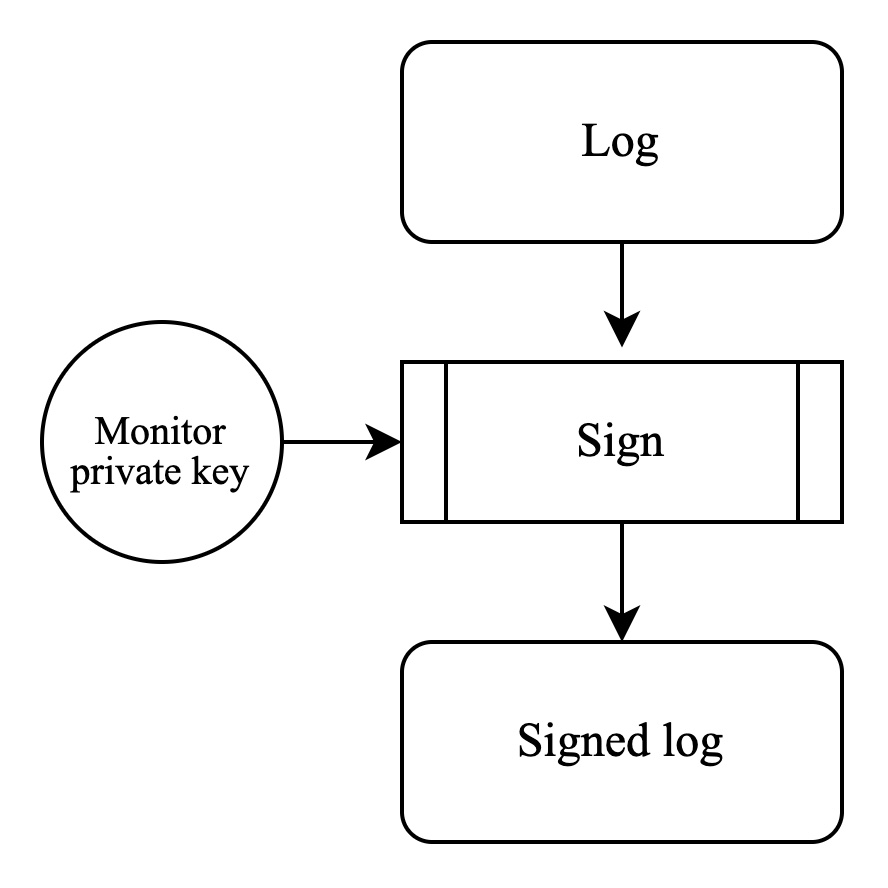
\includegraphics[scale=0.2]{../img/05/sign_logs.jpg}
        \centering
        \caption{A monitor needs to sign the access log with its private signing key.}
        \label{fig:signing}
    \end{subfigure}
    \begin{subfigure}
        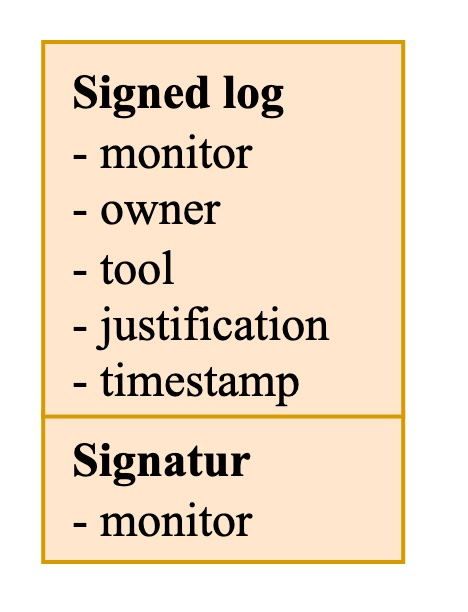
\includegraphics[scale=0.2]{../img/05/signed_log.jpg}
        \centering
        \caption{A \textit{signed log} is a JWS token containing the log data. It is signed by the monitor.}
        \label{fig:signed_log}
    \end{subfigure}
\end{figure}


\subsection{Encrypting logs}
\label{sec:encrypting}
The encryption of logs can be performed either by a monitor or the data owner.
The monitor initially encrypts the log for the data owner.
The data owner might decide to share the log with others.
This requires the re-encryption of the log.
The encryption algorithm requires a signed log and the set of users who are allowed to access the log as input parameters.
The encryption algorithm outputs a JWE token which can be decrypted by the specified users.

Internally, the encryption algorithm creates two JWS tokens.
They are called \textit{shared header} and \textit{shared log}.
Both are signed by the creator of the encrypted data (i.e. the entity that applies the encryption algorithm).
This is either the monitor creating the log or the data owner sharing the log.

The structure of a \textit{shared log} is visualized in figure~\ref{fig:shared_log}.
It contains the signed log (which was given as input to the encryption algorithm) as a nested JWS token.
It also contains the identity of the creator.
This allows decrypting users to request the public key needed to verify the signatures of the JWS tokens.
The \textit{shared log} is the final data structure being encrypted using hybrid encryption.

The structure of a \textit{shared header} is depicted in figure~\ref{fig:shared_header}.
It contains the set of receivers and the identity of the data owner.
This JWS token is not encrypted.
Rather, it is placed in the header of the JWE token.
This allows intermediate servers (e.g. the Overseer) to know which users can access a token and which user is allowed to modify a
\footnote{
    Consider the case where intermediate servers do not have this information.
    This implies that a server can not associate logs with users.
    From the perspective of the server all logs are encrypted data without meaningful information.
    If a user requests logs concerning him or her, the server must response with all logs stored in the system. 
    If the server, on the contrary, can associate logs with users, it can return exactly those logs which are intended for a particular user. 
    Since the header also includes the identity of the data owner, the server can also decide if a user is allowed to modify the encrypted log or not.
    Only the owner of a log is allowed to modify the encrypted log.
}.
Both, the \textit{shared header} and the \textit{shared log} are signed by the creator of the encrypted data.
To prevent a malicious entity to swap the \textit{shared header} with another valid header (e.g. from another encrypted log signed by the same creator), the \textit{shared header} and the \textit{shared log} must be linked together.
This is realized by including the same UUID, which is called \textit{shareID}, in both data structures.
A decrypting user can only trust a log if the \textit{shared header} and the \textit{shared log} are both signed by the claimed creator and if both contain the same \textit{shareID}.
\begin{figure}[h!]
\begin{subfigure}
    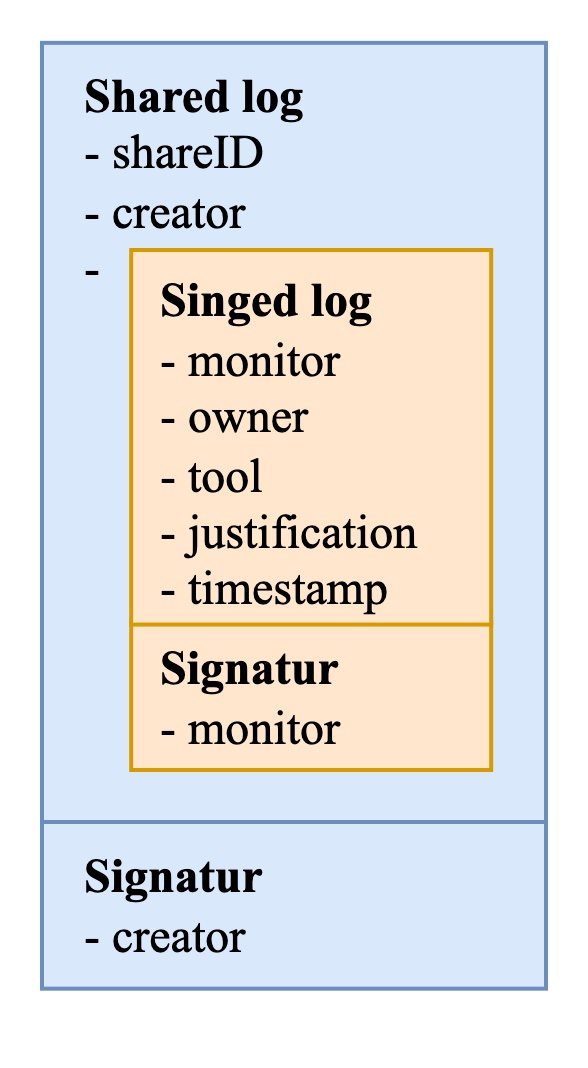
\includegraphics[scale=0.2]{../img/05/shared_log.jpg}
    \centering
    \caption{A shared log is a JWS token containing the nested \textit{signed log}. It is signed by the creator of the encrypted data (either the monitor or the data owner).}
    \label{fig:shared_log}
\end{subfigure}
\begin{subfigure}
    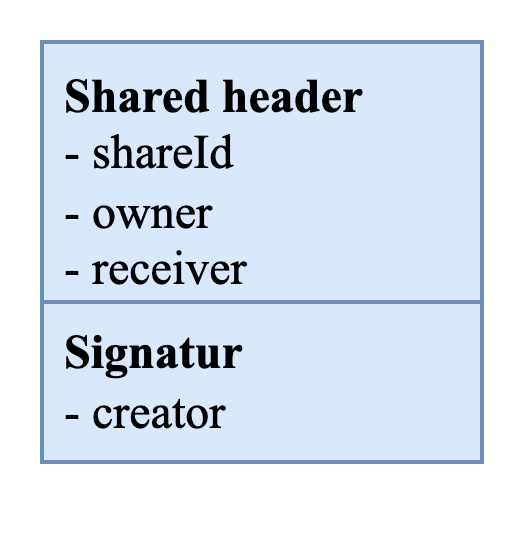
\includegraphics[scale=0.2]{../img/05/shared_header.jpg}
    \centering
    \caption{A shared header is a JWS token containing metadata of the sharing process. It is signed by the creator of the encrypted data (either the monitor or the data owner).}
    \label{fig:shared_header}
\end{subfigure}
\end{figure}

Once both JWS tokens, namely the \textit{shared header} and the \textit{shared log}, are cryptographically signed, they can be used to compute the final JWE token.
This is achieved by passing the \textit{shared log} as plaintext into the JWE encryption algorithm.
The \textit{share header} is passed into the protected header of the JWE algorithm.
The plaintext is encrypted with the authenticated encryption algorithm \verb|A256GCM| (symmetric encryption via 256-bit AES in Galois/Counter Mode).
The applied key-wrapping algorithm is \verb|ECDH-ES+A256KW|.
It is responsible for encrypting the symmetric key for authorized users (asymmetric encryption).
This algorithm establishes a Diffie-Hellman secret between the sender and receiver which is used to symmetrically encrypt the symmetric key using AES.
Details about this approach can be found in \cite[100]{Barker2017}.
Both algorithms are specified by the JSON Web Algorithm (JWA) specification~\cite{Jones2015}.
The whole encryption process is depicted in detail in \ref{app:encryption}.


\subsection{Decrypting logs}
\label{sec:decrypting}

The decryption algorithm takes a JWE token and a private decryption key as input.
To verify the different JWS tokens encoded within the JWE token, this algorithm needs to be able to dynamically resolve the identities of users to their public keys.

First of all, the JWE token is parsed into its ciphertext, header and encrypted keys.
The JWE-decryption algorithm is then applied to the JWE token.
This decrypts the ciphertext using the passed private decryption key.
To be more precise, it tries to decrypt any of the encrypted keys.
If this succeeds, the symmetric encryption key is accessible.
This allows the decryption of the symmetric ciphertext restoring the \textit{shared log}.
No decryption is necessary to access the \textit{shared header} because is stored in the protected header of the JWE.
Note that the structure of the \textit{shared log} and \textit{shared header} are depicted in figures \ref{fig:shared_log} and \ref{fig:shared_header}.

After successful decryption, the obtained JWS-tokens must be validated.
This is important to detect any misusage of the protocol.
It ensures that the identified security requirements are met.
If any of the following checks fail, the decryption must be aborted.

First of all, the decryption algorithm checks if the creator specified in the \textit{shared log} signed both, the \textit{shared log} and the \textit{shared header}.
It also needs to check if the specified \textit{shareIDs} are identical.
This ensures that claimed creator created both, the \textit{shared log} and the \textit{shared header} and that both are tied to each other.
Next, the algorithm needs to check if the identity of the decrypting user is part of the receivers specified in the \textit{shared header}.
If this holds, the decrypting user can be sure that the creator encrypted the log for him or her.
At this point, the nested \textit{signed log} can be extracted from the \textit{shared log}.
The structure of the \textit{signed log} is visualized in figure \ref{fig:signed_log}.
Since the \textit{signed log} is expected to be signed by the claimed monitor, the decryption algorithm needs to fetch the public key of the monitor and verify the signature of the \textit{signed log}.
If this check passes, the signatures of all JWS tokens have been validated.
Specifically, the decrypting user can be sure that the signed log was created by the claimed monitor.
Two further checks, however, are required.
First, the owner in the \textit{shared header} needs to be equal to the owner specified in the \textit{signed log}.
Note that the owner specified in the \textit{shared header} is used by the server to check which user can update encrypted logs.
This check ensures that the \textit{shared header} contains valid data and is not misformed.
Second, the creator of the \textit{shared log} needs to be either the owner of the log or the monitor of the log.

\section{Implemented Libraries}
\label{sec:implemented-libraries}

\subsection{Ts-It-Crypto}

\subsection{Py-It-Crypto}

\subsection{Go-It-Crypto}

\section{Toolchain modifications}
\label{sec:toolchain-modifications}


\end{document}
